\documentclass[../../Rapport RayTracer.tex]{subfiles}

\begin{document}

Pour parser notre fichier, nous avons besoin d'une classe servant en quelque sorte de chef d'orchestre. C'est la classe Automat. Elle possède un état courant, qui correspond à une figure dans le fichier pov, de type State. State est l'énumération des différentes figures possibles. Cette classe et cette énumération sont contenues dans le package povParser.


\begin{figure}[h!]
	\adjustbox{center}{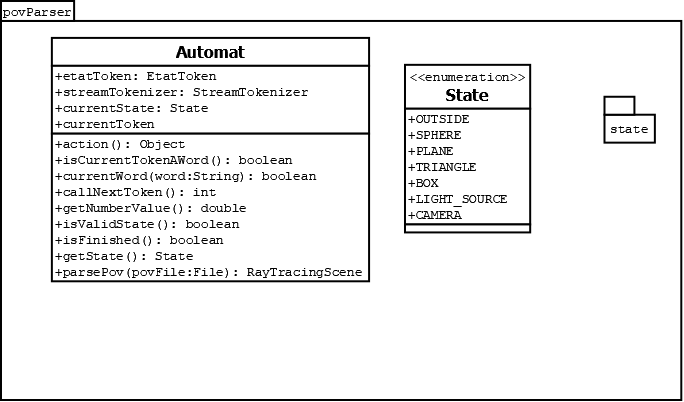
\includegraphics[width=0.75\textwidth]{diagrammes/package_povparser.png}}	
	\caption{Diagramme du package povParser}
	\label{diagrammePackagPovParser}
\end{figure}
\FloatBarrier

Le package state, quant à lui contient toutes les classes représentant des états, soit de figures (sphère, triangle, ...), la source de lumière, la caméra etc. Toutes les classes de ce package implémentent l'interface EtatToken. Chaque classe d'état possède sa propre énumération qui définit des contantes représentant des éléments de syntaxe. 

\begin{figure}[h!]
	\adjustbox{center}{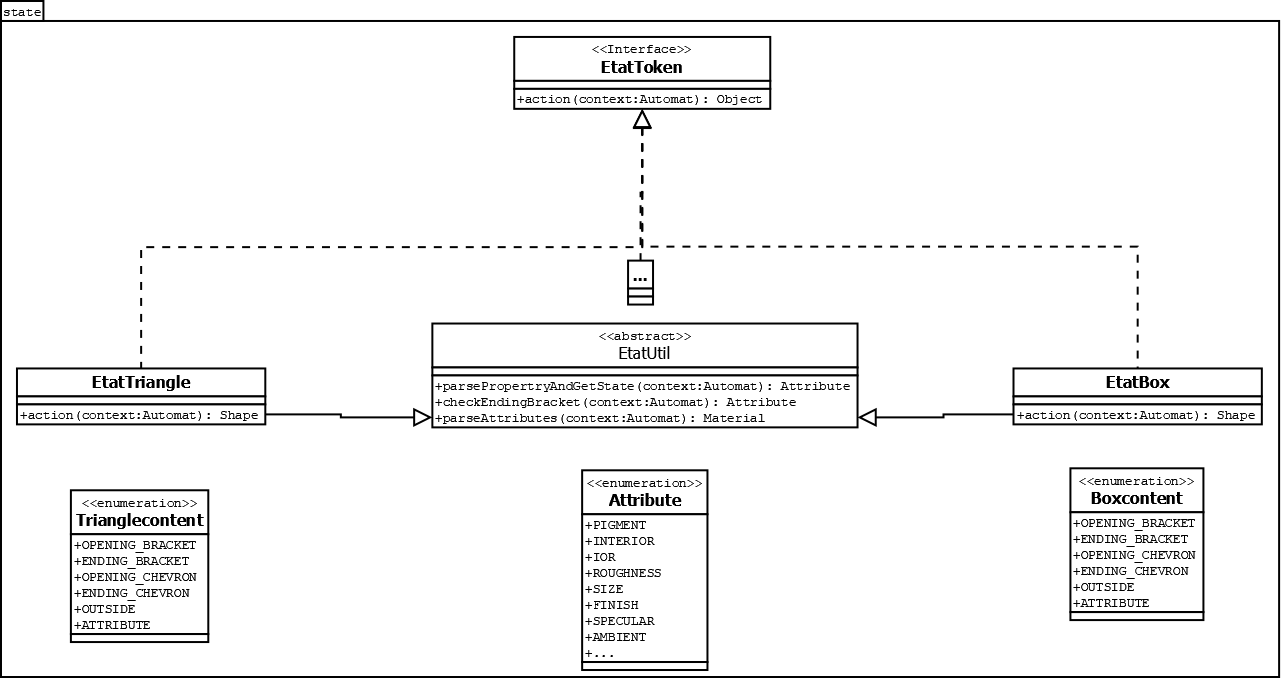
\includegraphics[width=1.25\textwidth]{diagrammes/package_state.png}}	
	\caption{Diagramme du package state}
	\label{diagrammePackagPovParser}
\end{figure}
\FloatBarrier

\end{document}